\documentclass[12pt compsoc]{article}
\usepackage{graphicx}
\graphicspath{ {./images/} } %if you have a folder with images, put the folder in directory and name it
\usepackage{subfig}
\usepackage[margin=2.5cm]{geometry}
\usepackage{listings}
\usepackage{hyperref}
\usepackage{amsmath}
\usepackage{color}
\usepackage{placeins}
\usepackage{float}


%%%%%%%%%%%%%%%%%%%%%%%%%%%%%%%%%%%%%%%%%%%%%%%%%%%%%%%%%%%%%%%%
%IMAGEIMAGEIMAGEIMAGEIMAGEIMAGEIMAGEIMAGEIMAGEIMAGEIMAGEIMAGEIMAGEIMAGEIMAGEIMAGEIMAGEIMAGEIMAGEIMAGE%
%%%%%%%%%%%%%%%%%%%%%%%%%%%%%%%%%%%%%%%%%%%%%%%%%%%%%%%%%%%%%%%%

%use this for standard images

%\begin{figure}[H]
%\centering
%\includegraphics[width=4in]{IMAGE_NAME}
%\caption{CAPTION HERE}
%\label{fig_LABEL_NAME}
%\end{figure}



%use this for side-by-side images, add more if you like to get 3 in a row....

%\begin{figure}[H]
%\centering
%\subfloat{\includegraphics[width=3in]{IMAGE_NAME}}
%\hspace{5mm}
%\subfloat{\includegraphics[width=3in]{IMAGE_NAME}}
%\caption{CAPTION HERE}
%\label{fig_LABEL_NAME}
%\end{figure}

%%%%%%%%%%%%%%%%%%%%%%%%%%%%%%%%%%%%%%%%%%%%%%%%%%%%%%%%%%%%%%%%
%TABLETABLETABLETABLETABLETABLETABLETABLETABLETABLETABLETABLETABLETABLETABLETABLETABLETABLETABLETABLETABLE%
%%%%%%%%%%%%%%%%%%%%%%%%%%%%%%%%%%%%%%%%%%%%%%%%%%%%%%%%%%%%%%%%

%\begin{table}[H]
%\centering
%\hspace{0cm}\begin{tabular}{| c | c |} %Add more columns here
%\hline
%Hex Value & Description\\
%\hline
%STUFF & STUFF\\
%\hline
%STUFF & STUFF\\
%\hline
%STUFF & STUFF\\
%\hline
%STUFF & STUFF\\
%\hline
%STUFF & STUFF\\
%\hline
%STUFF & STUFF\\
%\hline
%\end{tabular} 
%\caption{CAPTION HERE}
%\label{fig_LABEL_NAME}
%\end{table}




\begin{document}

\title{The Framework}

\author{Zach Levenberg}

\maketitle


\begin{figure}[H]
\centering
%\includegraphics[width=4in]{einstein.jpg}
\end{figure}

\begin{figure}[b!]
\centering
%\subfloat{\includegraphics[width = 4in]{SOE_logo.jpg}}
\end{figure}

\newpage

%%%%%%%%%%%%%%%%%%%%%%%%%%%%%%%%%%%%%%%%%%%%%%%%%%%%%%%%%%%%%%%%
%%%%%%%%%%%%%%%%%%%%%%%%%%%%%%%%%%%%%%%%%%%%%%%%%%%%%%%%%%%%%%%%
%%%%%%%%%%%%%%%%%%%%%%%%%%%%%%%%%%%%%%%%%%%%%%%%%%%%%%%%%%%%%%%%


\abstract{This paper explains how The Framework is implemented, and how to use it in an embedded system}
\newpage

\tableofcontents
\newpage

%%%%%%%%%%%%%%%%%%%%%%%%%%%%%%%%%%%%%%%%%%%%%%%%%%%%%%%%%%%%%%%%
%%%%%%%%%%%%%%%%%%%%%%%%%%%%%%%%%%%%%%%%%%%%%%%%%%%%%%%%%%%%%%%%
%%%%%%%%%%%%%%%%%%%%%%%%%%%%%%%%%%%%%%%%%%%%%%%%%%%%%%%%%%%%%%%%

\section{What is an RTOS?}

\subsection{Operating systems}
Most operating systems appear to allow multiple programs to execute at the same time. This is called multi-tasking. In reality, each processor core can only be running a single thread of execution at any given point in time. A part of the operating system called the scheduler is responsible for deciding which program to run when, and provides the illusion of simultaneous execution by rapidly switching between each program.

The type of an operating system is defined by how the scheduler decides which program to run when. For example, the scheduler used in a multi user operating system (such as Unix) will ensure each user gets a fair amount of the processing time. As another example, the scheduler in a desk top operating system (such as Windows) will try and ensure the computer remains responsive to its user.

\subsection{Embedded RTOS}
The scheduler in a Real Time Operating System (RTOS) is designed to provide a predictable (normally described as deterministic) execution pattern. This is particularly of interest to embedded systems as embedded systems often have real time requirements. A real time requirements is one that specifies that the embedded system must respond to a certain event within a strictly defined time (the deadline). A guarantee to meet real time requirements can only be made if the behavior of the operating system's scheduler can be predicted (and is therefore deterministic).

Traditional real time schedulers achieve determinism by allowing the user to assign a priority to each thread of execution. The scheduler then uses the priority to know which thread of execution to run next.
\\

Source: http://www.freertos.org/about-RTOS.html


%%%%%%%%%%%%%%%%%%%%%%%%%%%%%%%%%%%%%%%%%%%%%%%%%%%%%%%%%%%%%%%%
%%%%%%%%%%%%%%%%%%%%%%%%%%%%%%%%%%%%%%%%%%%%%%%%%%%%%%%%%%%%%%%%
%%%%%%%%%%%%%%%%%%%%%%%%%%%%%%%%%%%%%%%%%%%%%%%%%%%%%%%%%%%%%%%%

\section{The Bolt Motorbikes Framework}
\subsection{Intro}
The bolt framework is the system that all micro controllers in run as the base application. The Framework handles all initialization at startup, the scheduling and execution of services and tasks, and all timer related functions. The framework features a user configurable multi level priority queue for event handling. Events with a higher priority level will be processed before events with a lower priority. Events can be posted to any service and the service will be called automatically by the framework. The framework timer is guaranteed down to 1ms.

\subsection{Common Terms}
Framework: The lowest level firmware that abstracts away system operating details and runs the user application.
\\\\
Service: An routine that responds to Events. A service can be simple, or complex with many states. Services are designed to be used as State Machines, but may only contain a single state if desired.
\\\\
Event: An event is a definition of an action that occurs in the real world. An Event may be a button press, or a timer expiring. It can also signify a message that has been received.
\\\\
State Machine: A state machine is essentially a road map of behaviors that change due to internal or external events. There is no limit to the complexity or size of a state machine.

\subsection{Quickstart}

 To start the  framework, the system clock must already be initialized. A single call to Framework Run must be made with the system clock frequency as the only argument. Once running, the framework will post an INIT\_EVENT to each of the services. Each service *should* have a section for initialization code that is related to that service. At this time, the TaskRunner is started and begins running at a frequency of 1000Hz (1ms). If any events are found, the event will be posted to the specified event, and the service will be called with the Event as the argument. See Figure \ref{fig_frameworkDiagram} for the flow of the framework.
 
\begin{figure}[H]
\centering
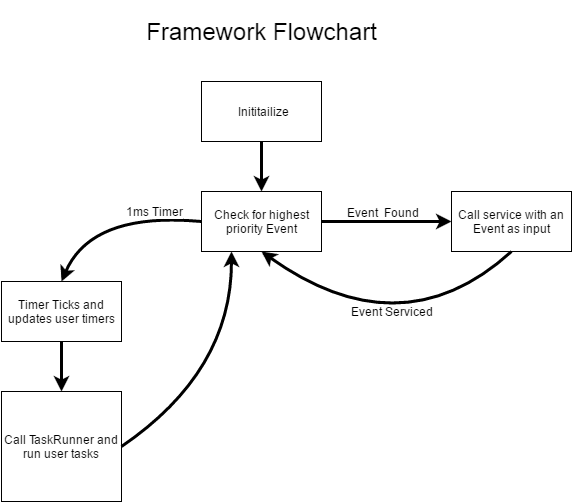
\includegraphics[width=6in]{FrameworkDiagram.PNG}
\caption{Framework Flowchart Diagram}
\label{fig_frameworkDiagram}
\end{figure}


\section{Configuration}
\subsection{Library Structure}
All projects that use this Framework must follow this structure. The files ``Framework.h'' and ``Framework.c'' must be included in the project directory, or in a user specified location as a reference. These files must not be modified! Changing anything in these files could cause undetermined behavior and will not be supported by the creators of this framework.
\subsection{Framwork\_Configure.h}
All projects that use this Framework must include a unique, project-specific copy of ``Framework\_Configure.h''. This file is expected by ``Framework.c'' and must be included.
framework.
\subsubsection{Events}
In ``Framework\_Configure.h'', the user may specify Events, to be used throughout the project. To add an event, simply follow the format as the default Events are written in. For example:

\begin{verbatim}
#define EVENT_LIST(EVENT) \
EVENT(NO_EVENT) \
EVENT(FAIL_EVENT) /* Runtime failure in the state machine */ \
EVENT(INIT_EVENT) /* The transition out of init state */ \
EVENT(ENTRY_EVENT) /* Put any entry code for a state when this state is thrown */ \
EVENT(EXIT_EVENT) /* Exit code for states triggered by this event */ \
EVENT(TIMEUP_EVENT) /* The timer-up event for timers */ \
EVENT(DEBUG_MESSAGE_EVENT) /*Incoming debug message*/ 
EVENT(CUSTOM_EVENT) /*Just follow this format to create more events!*/ 
\end{verbatim}

\subsubsection{Priorities}

The User may also specify the number of Priority Levels and the Priority Queue Depth. Note that Timers and the TaskRunner (more on this later) always have the highest priority, because timing is critical.

\begin{verbatim}
typedef enum _priority {
    FRAMEWORK_PRIORITY_1,
    FRAMEWORK_PRIORITY_2,
    FRAMEWORK_PRIORITY_3,
    CUSTOM_PRIORITY_HERE,
    FRAMEWORK_PRIORITY_LEVELS //Make sure this is always last
} FRAMEWORK_priority_E;

#define FRAMEWORK_QUEUE_SIZE 4 //Don't make the queue larger than 8
\end{verbatim}•

\subsubsection{Services}
Final, the user may also specify more services. Follow this format when creating new services.

\begin{verbatim}
/*Put the name of each service*/
#define SERVICE_LIST(SERVICE) \
SERVICE(myCoolNewService) /*Main state machine, This is always first (the default Service)*/ \
SERVICE(debuggerService) /*This debugger service handles the Uart interface to PC*/ \

/* file name of each service IN THE SAME ORDER AS ABOVE*/
#define SERVICE_1 "myCoolNewService.h"
#define SERVICE_2 "debuggerService.h"
//#define SERVICE_3
//#define SERVICE_4 
//#define SERVICE_5 
//#define SERVICE_6 
//#define SERVICE_7 
//#define SERVICE_8 
\end{verbatim}•

As you define more services, be sure to uncomment each \#define, and make sure the two lists ``agree'' in that their service name and file name are in the same order. The file name and service may be different, but the service name MUST be the name of the function in the service.

\subsection{Framwork\_TaskRunner.c}
Another required file for this project is Framwork\_TaskRunner.c. The file must have the following functions or the framework will not compile:

\begin{verbatim}
void FRAMEWORK_TASKRUNNER_init(void) {
}

inline void FRAMEWORK_TASKRUNNER_1ms(void) {
}

inline void FRAMEWORK_TASKRUNNER_10ms(void) {
}

inline void FRAMEWORK_TASKRUNNER_100ms(void) {
}

inline void FRAMEWORK_TASKRUNNER_1000ms(void) {
}
\end{verbatim}•

This section is very simple and very useful. The user may put any code here that they want to run continuously at the specified rate. Simple counters may be used to obtain other denominations. This is a great place to put functions that check for events. For example, a function that checks if a button has been pressed, or if a message has been recieved. This is where most events will originate from.

\section{Events and Services}
\subsection{Writing a service}
A service must consist of a .h file and a .c file. The function prototype must follow the following format:

\begin{verbatim}
Event myCoolNewService(Event ThisEvent);
\end{verbatim}•

That is to say that the function takes an Event as an argument, and returns an Event. Whatever happens inside the function is completely up to the user. It is, however, recommended to follow the format of the Template Service. Note that the name of the function is the same as defined in ``Framework\_Configure.h''!

The user may decide to add other public helper functions to the service, but only one is required.

And finally, the Event datatype is defined in ``Framework\_Configure.h'' but it may not be modified.

\begin{verbatim}
/* The Event type */
typedef struct Event_t {
    FRAMEWORK_eventType_E EventType;
    uint16_t EventParam;
    FRAMEWORK_priority_E EventPriority;
    FRAMEWORK_serviceType_E Service;
} Event;
\end{verbatim}•

An Event must contain an EventType from the list of Event you defined above. It may optionally contain a 16bit parameter of the user's choosing. It may optionally contain a Priority, the default priority is 0 (lowest). It may optionally contain a service, the default service is the first one listed in the service list The service name to use in this field will always be the myCoolNewSevice\_SERVICE, due to variable name and function name collisions. It is always recommended to explicitly state all of the parameters of the Event.

\section{Framework Functions}

\subsection{FRAMEWORK\_run}
\begin{verbatim}

/**
 * Main framework run function
 * @param clockFreq: System Frequency in Hz
 * @return 

uint8_t FRAMEWORK_run(uint32_t clockFreq);
\end{verbatim}•


\subsection{FRAMEWORK\_postEvent}
\begin{verbatim}
/**
 * Post an event into the priority queue
 * @param thisEvent: contains type, param, service, and priority
 * @return 
 */
uint8_t FRAMEWORK_postEvent(Event thisEvent);
\end{verbatim}

\subsection{FRAMEWORK\_Debug}
\begin{verbatim}
/**
 * Enable or disable debug messages
 * @param state Enabled (1) or Disabled (0)
 */
void FRAMEWORK_Debug(uint8_t state);
\end{verbatim}

\subsection{FRAMEWORK\_resetTimeNow}
\begin{verbatim}
/**
 * Resets the 45-day freerunning timer, should be performed periodically or on 
 * system wake from sleep
 */
void FRAMEWORK_resetTimeNow(void);
\end{verbatim}

\subsection{FRAMEWORK\_getTimeNow}
\begin{verbatim}
/**
 * Returns the value of the freerunning timer in milliseconds
 * @return 
 */
uint32_t FRAMEWORK_getTimeNow(void);
\end{verbatim}

\subsection{FRAMEWORK\_timerSet}
\begin{verbatim}
/**
 * Sets a one-shot timer and throws a TIMEUP Event upon completion
 * @param thisTimer: Timer number to set (0-15)
 * @param time: the time in milliseconds
 * @param service: the service in which the TIMEUP Event is posted to.
 * @param Mode: the type of timer to run (continuous or one-shot)
 */
void FRAMEWORK_timerSet(FRAMEWORK_timerNumber_E thisTimer, uint16_t time, FRAMEWORK_serviceType_E service, FRAMEWORK_timerMode_E Mode);
\end{verbatim}

\subsection{FRAMEWORK\_timerStop}
\begin{verbatim}
/**
 * Halts a timer before it expires
 * @param thisTimer: timer to be halted (0-15)
 */
void FRAMEWORK_timerStop(FRAMEWORK_timerNumber_E thisTimer);
\end{verbatim}

\subsection{FRAMEWORK\_timerResume}
\begin{verbatim}
/**
 * Resumes a timer that has been halted
 * @param thisTimer: timer to be resumed (0-15)
 */
void FRAMEWORK_timerResume(FRAMEWORK_timerNumber_E thisTimer);


\end{verbatim}•


\end{document}